\documentclass[a4paper]{article}    % define document layout
%\documentclass[draft]{article}     % use draft option in packages
%-----------------------------
% preamble
%-----------------------------
\usepackage[sumlimits,]{amsmath}    % math equations and formulas
\usepackage[utf8]{inputenc}         % use UTF-8 encoding
\usepackage[english]{babel}         % use English language
\usepackage{graphicx}               % insert images
%\usepackage[draft]{graphicx}        % do not render figures
\usepackage{subcaption}             % multiple images in one figure
\usepackage{hyperref}               % hyperlinks
\usepackage{float}                  % floating objects (figures, tables)
\usepackage{geometry}               % page size and margins
\geometry{a4paper, margin=1in}      % margins
\usepackage{ragged2e}               % text alignment
\usepackage[table]{xcolor}          % change cell color in tables
%\usepackage{multirow}               % merge rows in table

\graphicspath{                      % path for figures
    {../figures/} 
}

%-----------------------------
% body
%-----------------------------
\begin{document}

\begin{figure}
    \centering
    % UNICAMP logo
    \begin{subfigure}{0.45\textwidth}
        \centering
        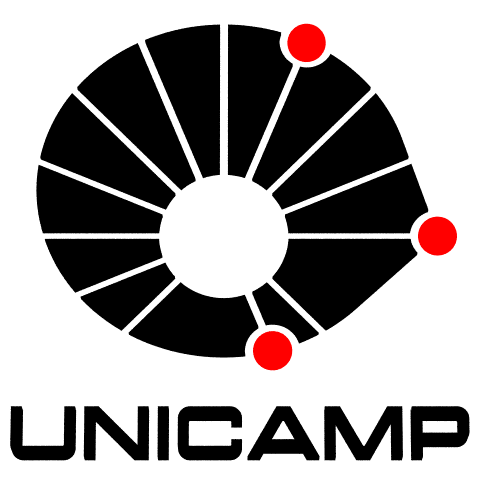
\includegraphics[width=1.5cm]{unicamp}
%        \label{fig:unicamp}
    \end{subfigure}
    \hfill
    % FEEC logo
    \begin{subfigure}{0.45\textwidth}
        \centering
        
\includegraphics[width=1.5cm]{feec}
%        \label{fig:feec}
    \end{subfigure}
\end{figure}

\title{
    \vspace{5cm}
    IA353A - Neural Networks\\
    EFC3
    \vspace{1cm}
}
\author{
    Rafael Claro Ito\\
    (R.A.: 118430)
    \vspace{11cm}
}
%R.A.: 118430
%ito.rafael@gmail.com
\date{July 2020}
\maketitle
\newpage

%=================================================
\section{Source files}
%=================================================

\paragraph{The Jupyter notebook with the code used to generate the plots and results presented in this report, all figures showed here and even the \LaTeX \space source code used to generate this PDF can be found at the following GitHub repository:}

\begin{center}
    {\url{https://github.com/ito-rafael/IA353A-NeuralNetworks-1s2020}}
\end{center}

%=================================================
\section{Q5 - Autoencoder}
%=================================================

%-------------------------------------------------
\subsection{1) Improve classes distribution}
%-------------------------------------------------

\href{https://colab.research.google.com/drive/1N7auSaSqYvORHTUK031ZfX4upoA38-hI?usp=sharing}{https://colab.research.google.com/drive/1N7auSaSqYvORHTUK031ZfX4upoA38-hI?usp=sharing}

%=================================================
\end{document}

